% A Poisson process of rate 2 on [0,10] and its thinning with p=1/3. Generated by a short script.
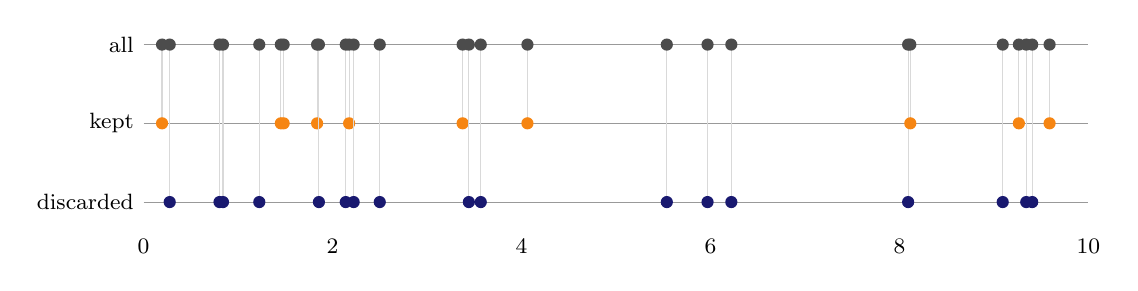
\begin{tikzpicture}[x=1.2cm,y=1cm,every node/.style={font=\footnotesize}]
\draw[black!40] (0,2)--(10,2);
\node[left] at (0,2) {all};
\draw[black!40] (0,1)--(10,1);
\node[left] at (0,1) {kept};
\draw[black!40] (0,0)--(10,0);
\node[left] at (0,0) {discarded};
\draw[black!15] (0.196,2)--(0.196,1);
\fill[black!70] (0.196,2) circle (2.2pt);
\fill[BurntOrange] (0.196,1) circle (2.2pt);
\draw[black!15] (0.277,2)--(0.277,0);
\fill[black!70] (0.277,2) circle (2.2pt);
\fill[MidnightBlue] (0.277,0) circle (2.2pt);
\draw[black!15] (0.804,2)--(0.804,0);
\fill[black!70] (0.804,2) circle (2.2pt);
\fill[MidnightBlue] (0.804,0) circle (2.2pt);
\draw[black!15] (0.841,2)--(0.841,0);
\fill[black!70] (0.841,2) circle (2.2pt);
\fill[MidnightBlue] (0.841,0) circle (2.2pt);
\draw[black!15] (1.225,2)--(1.225,0);
\fill[black!70] (1.225,2) circle (2.2pt);
\fill[MidnightBlue] (1.225,0) circle (2.2pt);
\draw[black!15] (1.453,2)--(1.453,1);
\fill[black!70] (1.453,2) circle (2.2pt);
\fill[BurntOrange] (1.453,1) circle (2.2pt);
\draw[black!15] (1.483,2)--(1.483,1);
\fill[black!70] (1.483,2) circle (2.2pt);
\fill[BurntOrange] (1.483,1) circle (2.2pt);
\draw[black!15] (1.837,2)--(1.837,1);
\fill[black!70] (1.837,2) circle (2.2pt);
\fill[BurntOrange] (1.837,1) circle (2.2pt);
\draw[black!15] (1.856,2)--(1.856,0);
\fill[black!70] (1.856,2) circle (2.2pt);
\fill[MidnightBlue] (1.856,0) circle (2.2pt);
\draw[black!15] (2.140,2)--(2.140,0);
\fill[black!70] (2.140,2) circle (2.2pt);
\fill[MidnightBlue] (2.140,0) circle (2.2pt);
\draw[black!15] (2.176,2)--(2.176,1);
\fill[black!70] (2.176,2) circle (2.2pt);
\fill[BurntOrange] (2.176,1) circle (2.2pt);
\draw[black!15] (2.224,2)--(2.224,0);
\fill[black!70] (2.224,2) circle (2.2pt);
\fill[MidnightBlue] (2.224,0) circle (2.2pt);
\draw[black!15] (2.500,2)--(2.500,0);
\fill[black!70] (2.500,2) circle (2.2pt);
\fill[MidnightBlue] (2.500,0) circle (2.2pt);
\draw[black!15] (3.377,2)--(3.377,1);
\fill[black!70] (3.377,2) circle (2.2pt);
\fill[BurntOrange] (3.377,1) circle (2.2pt);
\draw[black!15] (3.443,2)--(3.443,0);
\fill[black!70] (3.443,2) circle (2.2pt);
\fill[MidnightBlue] (3.443,0) circle (2.2pt);
\draw[black!15] (3.569,2)--(3.569,0);
\fill[black!70] (3.569,2) circle (2.2pt);
\fill[MidnightBlue] (3.569,0) circle (2.2pt);
\draw[black!15] (4.063,2)--(4.063,1);
\fill[black!70] (4.063,2) circle (2.2pt);
\fill[BurntOrange] (4.063,1) circle (2.2pt);
\draw[black!15] (5.538,2)--(5.538,0);
\fill[black!70] (5.538,2) circle (2.2pt);
\fill[MidnightBlue] (5.538,0) circle (2.2pt);
\draw[black!15] (5.969,2)--(5.969,0);
\fill[black!70] (5.969,2) circle (2.2pt);
\fill[MidnightBlue] (5.969,0) circle (2.2pt);
\draw[black!15] (6.221,2)--(6.221,0);
\fill[black!70] (6.221,2) circle (2.2pt);
\fill[MidnightBlue] (6.221,0) circle (2.2pt);
\draw[black!15] (8.092,2)--(8.092,0);
\fill[black!70] (8.092,2) circle (2.2pt);
\fill[MidnightBlue] (8.092,0) circle (2.2pt);
\draw[black!15] (8.115,2)--(8.115,1);
\fill[black!70] (8.115,2) circle (2.2pt);
\fill[BurntOrange] (8.115,1) circle (2.2pt);
\draw[black!15] (9.093,2)--(9.093,0);
\fill[black!70] (9.093,2) circle (2.2pt);
\fill[MidnightBlue] (9.093,0) circle (2.2pt);
\draw[black!15] (9.264,2)--(9.264,1);
\fill[black!70] (9.264,2) circle (2.2pt);
\fill[BurntOrange] (9.264,1) circle (2.2pt);
\draw[black!15] (9.342,2)--(9.342,0);
\fill[black!70] (9.342,2) circle (2.2pt);
\fill[MidnightBlue] (9.342,0) circle (2.2pt);
\draw[black!15] (9.405,2)--(9.405,0);
\fill[black!70] (9.405,2) circle (2.2pt);
\fill[MidnightBlue] (9.405,0) circle (2.2pt);
\draw[black!15] (9.589,2)--(9.589,1);
\fill[black!70] (9.589,2) circle (2.2pt);
\fill[BurntOrange] (9.589,1) circle (2.2pt);
\draw (0,-0.35) node[below] {$0$};
\draw (2,-0.35) node[below] {$2$};
\draw (4,-0.35) node[below] {$4$};
\draw (6,-0.35) node[below] {$6$};
\draw (8,-0.35) node[below] {$8$};
\draw (10,-0.35) node[below] {$10$};
\end{tikzpicture}
